%!TEX root = report.tex

\chapter{Prototyp Implementierung}
\label{cha:implementierung}

In der Referenzimplementierung von \dg verwenden wir die ANTLR Syntax zur formalen Definition unserer Sprache. Darauf aufbauen verwenden wir den von ANTLR bereitgestellten Parser und Lexer zum das in \dg geschriebene Spiel zu erfassen. \\

    \begin{figure}[ht]
    	\centering
        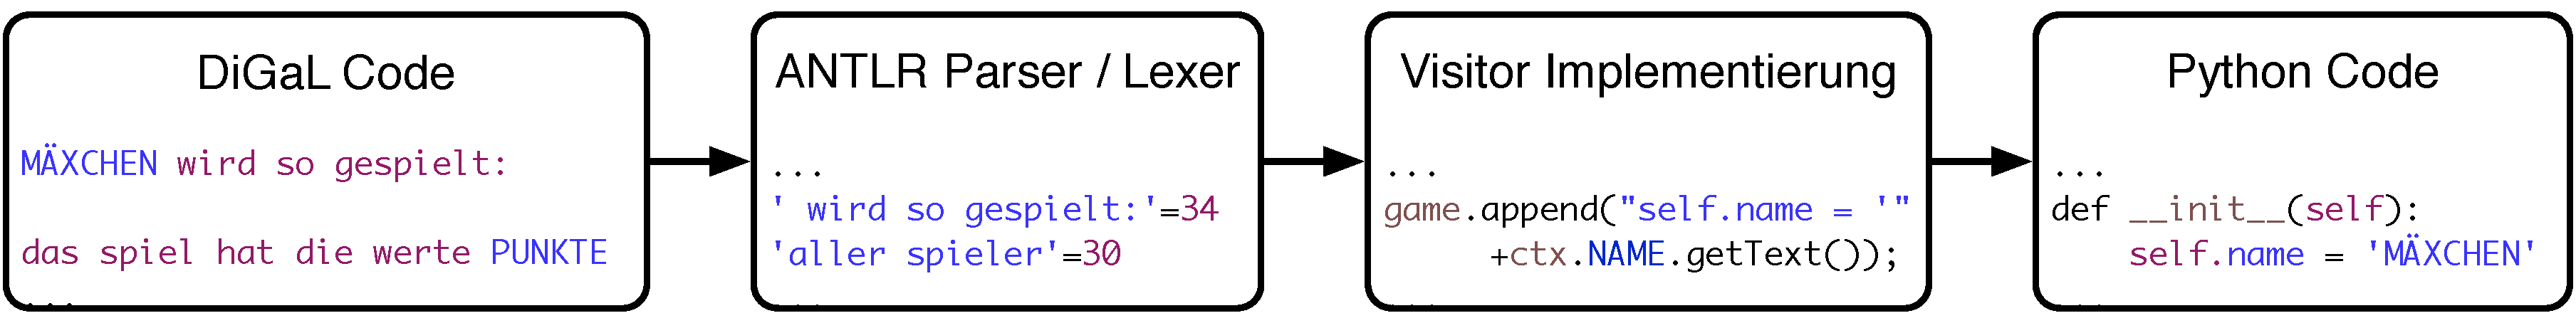
\includegraphics[width=\textwidth]{Flow.pdf}
    	\caption{Ablauf der Kompilation eines DiGaL Programmes}
    	\label{flow}
    \end{figure}

Um sicherzustellen, dass die mit \dg geschriebenen Spiele portabel sind, haben wir uns zum Ziel gesetzt möglichst wenige Abhängigkeiten vorauszusetzen. 
Ein Kriterium war dabei, dass die Ausführung des Codes nur mit der Standardbibliothek einer Zielsprache funktioniert. Wir haben uns deswegen für eine Kompilation der Sprache entschieden, und verzichten für den Endanwender auf die Installation von ANTLR. Als Zielsprache wählten wir Python, das Syntaktisch kompakt zu programmieren ist und inhärente Konzepte unserer Sprache unterstützt (Objektorientiertheit, Funktionale Programmierung). 

Zur Generierung des Python Codes haben wir uns für das Visitorpattern entschieden. Die Entscheidung gründet auf die Simplizität einer Implementierung dieses Patterns, das uns als lernende ANTLR Spielentwickler nur noch abverlangt die vorgegebenen Methoden zu implementieren und uns so auf das wesentlich zu konzentrieren. 

\section{Python Framework} % (fold)
\label{sec:python_framework}
    
    Zusammen mit der Definition der Grammatik haben wir generische Methoden ausgearbeitet. Die vorhanden Methoden lassen sich in zwei Klassen differenzieren: Generische Methoden, die in vielen Würfelspielen verwendet werden; Methoden die zur Interaktion mit den Mitspielern und zur Repräsentation von Daten gegenüber diesen nötig sind. Die zweite Gruppe ergibt sich nicht aus der Domäne selbst, sondern folgt aus der nötigen Mensch-Maschine Kommunikation (Ausgaben auf der Kommandozeile).
    
    \begin{figure}[ht]
    	\centering
        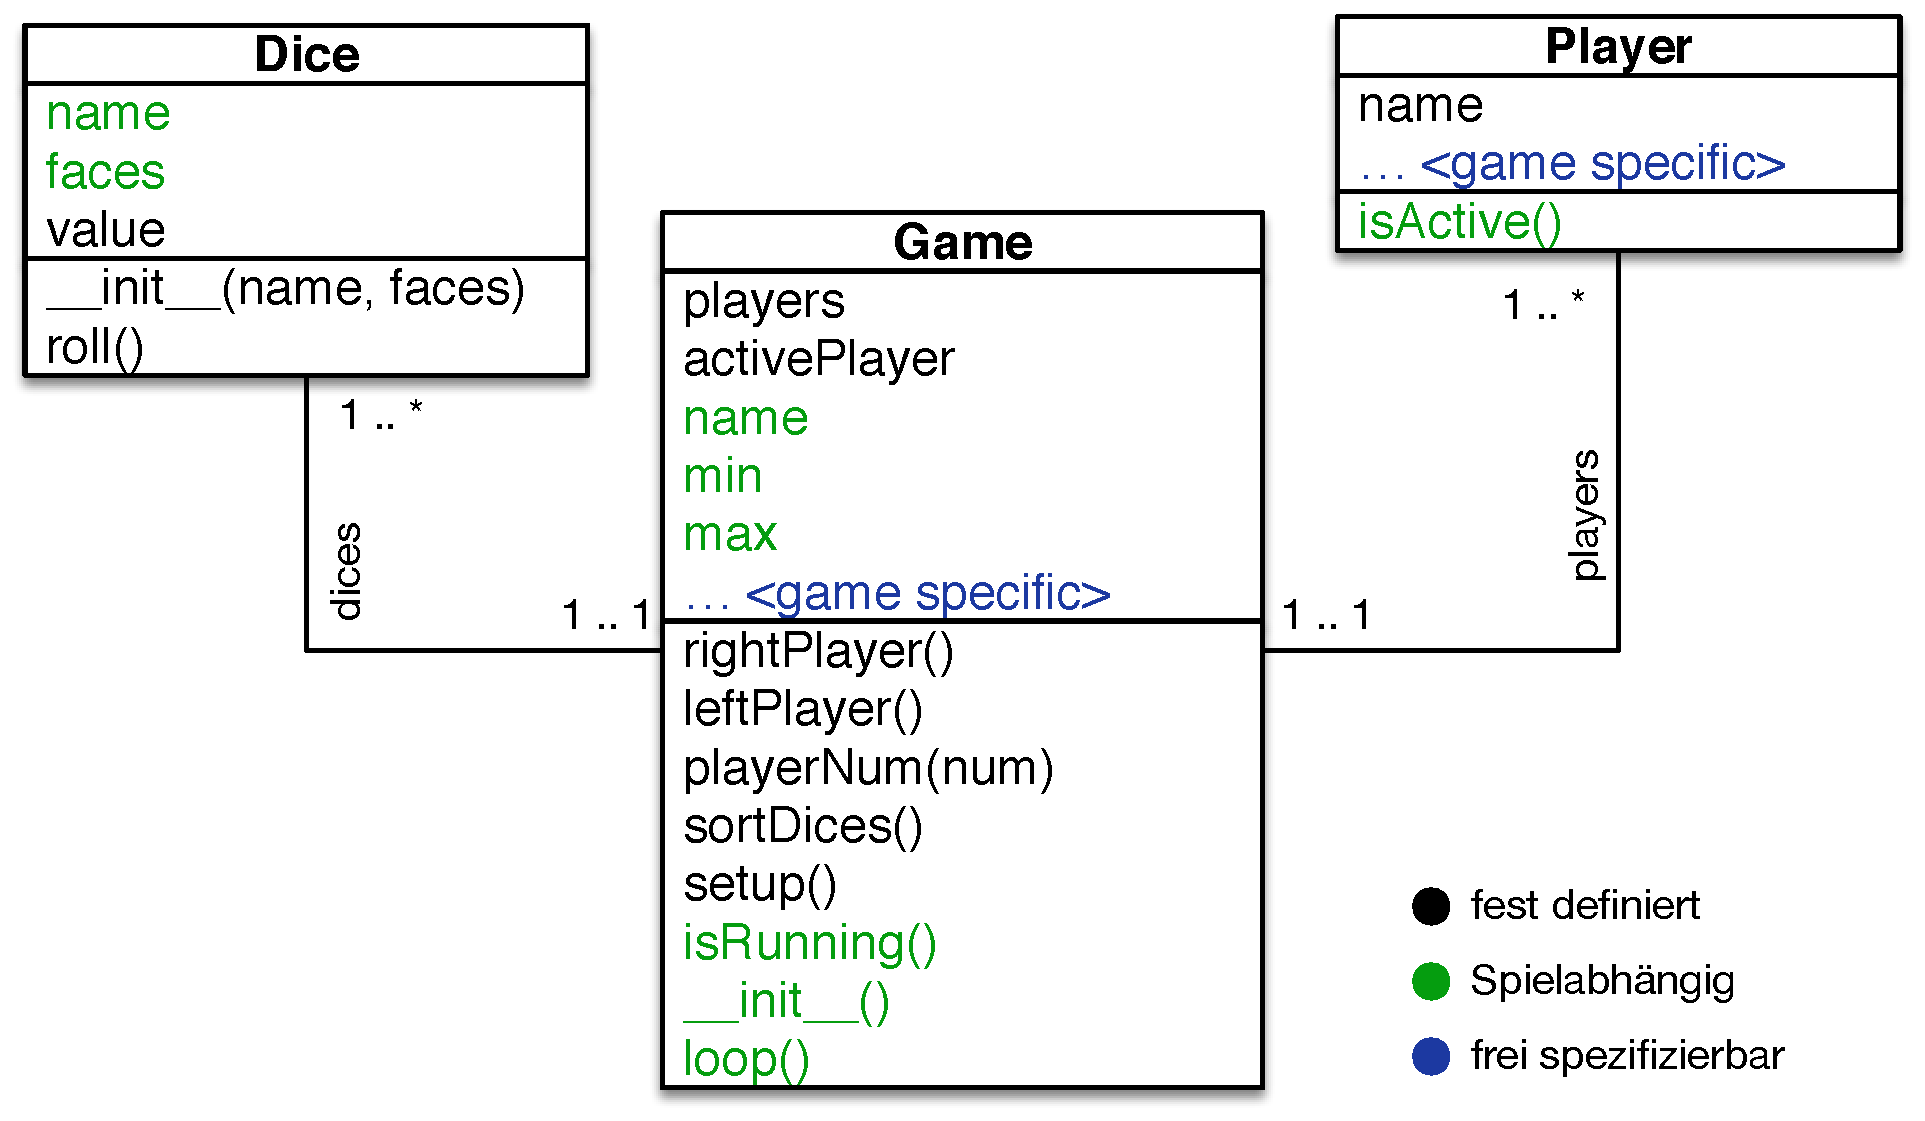
\includegraphics[width=0.8\textwidth]{Python-UML.pdf}
    	\caption{Klassendesign des Python Frameworks}
    	\label{python-uml}
    \end{figure}
    
    Die Domänenspezifischen Methoden können direkt aus der Sprache verwendet werden und entsprechen den verwendbaren Anweisungen (\texttt{würfelt mit <würfeln>}).
    
\section{Interne Datenrepräsentation} % (fold)
\label{sec:interne_datenreprasentation}
    Wie in den oben Abschnitten erwähnt, verwenden wir für die Implementierung Konstrukte unserer Zielsprache. Der objektorientierte Ansatz von \dg zeigt sich hier in der Umsetzung in Klassen für Spieler, Würfel und das Spiel selbst. Bei der Übersetzung eines Spiels werden Teile der gegebenen Klassen durch die vom Spielentwickler spezifizierten Eigenschaften des Spiels ergänzt. Beispiel dafür sind die Spieler, denen durch den Spielentwickler neuen Felder hinzugefügt werden können.Die Würfelklasse hingegen ist nicht erweiterbar, sondern wird nur durch die Implementierung der Spielklassen verschieden initialisiert.
    
    Die Spielklasse enthält die Initialisierung und den Ablauf des Spiels und ist die zentrale Klasse. Die Klasse enthält einige generische Methoden, die nicht individualisierbar sind und in der Sprache zur Verfügung stehen (\texttt{leftPlayer()}, \texttt{rightPlayer()}, \texttt{sortDices()}, ...). In Kontrast dazu bildet die \texttt{loop()}-Methode den Spielablauf ab und wird vom Entwickler frei definiert.
% section interne_datenreprasentation (end)
    
% section python_framework (end)

\section{Compilerimplementierungen}
\label{sec:compilerimplementierungen}
	Da die Implementierung recht umfangreich ist kann sie hier nicht vollständig angegeben werden. Daher beschränken wir uns hier auf einige Beispiele.
	
dg wurde so konzipiert, dass alle Domänenspezifischen Konzepte, wie sie oben beschrieben sind, direkt abgebildet werden können. Auch in der Pythonumsetzung haben wir versucht dies beizubehalten, und die Konzepte von \dg soweit wie möglich direkt in Python umzusetzen. Grundoperationen wie \texttt{+, -, *, größer, kleiner, gleich, ...} haben direkt in ihren entsprechenden Pythonoperatoren umgesetzt. Gleiches gilt für die Zuweisung. Diese kann in \dg zwar syntaktisch unterschiedlich sein, in Python wird daraus aber immer eine einfache Zuweisung.
	
		Des weiteren haben wir einige Abstraktionen vorgenommen, um die Paradigmen aus der Domäne umzusetzen. Als Beispiel sei folgender Code gegeben:
\begin{lstlisting}
wenn würfel A gleich 2 ...
\end{lstlisting}
		In konventionellen Programmiersprachen wäre diese Operation nicht ohne weiteres möglich, da ein Vergleich zwischen einem selbst definierten Objekt und einer Zahl zunächst nicht definiert ist. Im Bezug auf die Domäne ist dieser Ausdruck jedoch sinnvoll, da damit implizit gemeint ist, dass der gewürfelte Wert, also eine Zahl mit einer anderen verglichen werden soll. Diesen Umstand haben wir so gelöst, dass ein logischer Vergleich oder eine arithmetische Operation mit Würfeln immer als Operation auf dem entsprechenden gewürfelten Wert zu verstehen ist. Im Code sieht das wie folgt aus:

\begin{lstlisting}
if [dice for dice in self.dices if dice.name == 'A'].value == 2 ...
\end{lstlisting}
Diese Idee haben wir versucht so weit wie möglich umzusetzen. Sie findet sich beispielsweise in der referenzierung des nächsten Spielers wieder. Hier genügt es in \dg zum Beispiel das Schlüsselwort \texttt{linker spieler} zu verwenden. Diese Abstraktion haben wir in Python so umgesetzt, dass der Index der Liste, in dem Spieler gespeichert sind, um ein dekrementiert wird.

Weiterhin soll hier auf die Implementierung der Methode \texttt{isRunning()} eingegangen werden. Diese repräsentiert die Bedingung, die der Entwickler festlegen kann. Sie bestimmt, ob ein Spiel noch läuft oder nicht. Beispielsweise kann ein Spiel nach $n$ Runden zu Ende sein.

\begin{lstlisting}[label={lst:ODD}]
ODD wird so gespielt:

das spiel hat den wert RUNDEN ist 5.
...
das spiel läuft solange RUNDEN größer 0.
...
\end{lstlisting}
	Im oberen Listing wird beispielsweise die globale Variable \texttt{RUNDEN} definiert und als Bedingung festgelegt, dass ein Spiel solange läuft, solange \texttt{RUNDEN größer 5} gilt. Das heißt das Spiel läuft fünf Runden. Im kompilierten Pythoncode sieht das wie folgt aus:
\begin{lstlisting}[language=Python]
def isRunning(self): return (self.RUNDEN > 0)
\end{lstlisting}
Diese Methode hat eine weitere Besonderheit. Wird keine Bedingung festgelegt, weil ein Spiel beispielsweise kein deterministisches Ende hat, sondern von Fall zu Fall unterschiedlich ist, hat die Funktion einen Standardfall, bei dem immer \texttt{true} zurückgegeben wird. In diesem Fall muss sich der Entwickler aber selbst darum kümmern, das Spiel mit den Schlüsselwort \texttt{das spiel ist zu ende.} zu beenden. Methoden dieser Art, also die gegeben sein müssen, aber vom Nutzer gefüllt werden können, gibt es noch weitere, beispielsweise die Funktion \texttt{isActive()}, die nach einer von Entwickler definierten Bedingung entscheidet, ob ein Spieler aktiv ist oder nicht.


\section{Erfüllung der geforderten Sprachqualitäten} % (fold)
\label{sec:erfullung_der_geforderten_sprachqualitaten}

% section erfullung_der_geforderten_sprachqualitaten (end)

\section{Mögliche Erweiterungen} % (fold)
\label{sec:mogliche_erweiterungen}

% section mogliche_erweiterungen (end)












